%% Intended to be included into a larger document
\chapter{Related Work}
\label{cha:related-work}

This chapter examines related research in this area. The related work on serious games and the recent development of gamification is discussed in Section 2.1. Section 2.2 looks at the applications of ``serious game'' in the sustainability context. Finally, Section 2.3 and 2.4 examines the serious game framework and its assessment.

%% TODO: add more serious game examples
\section {Serious Games and Gamification}

A Serious game is ``a game designed for a primary purpose other than pure entertainment'' \cite {WikipediaSeriousGame}. It includes categories such as educational games and advergames (advertising), political games, and training game (also known as game-learning). Zyda \cite{Zyda2005} defines serious game is ``a mental contest, played with a computer in accordance with specific rules that uses entertainment to further government or corporate training, education, health, etc''.

One prominent example is Foldit \cite {khatib2011crystal}, a multiplayer online game which helps solving problems that computers can not solve very well, in this case, online gamers around the world together were able to do what biochemists have been trying to do for a decade: decipher the structure of a protein that is key to the way HIV multiplies. Figure \ref{fig:foldit} shows a screen shot of the Foldit game.

\begin{figure}[htbp]
	\centering
		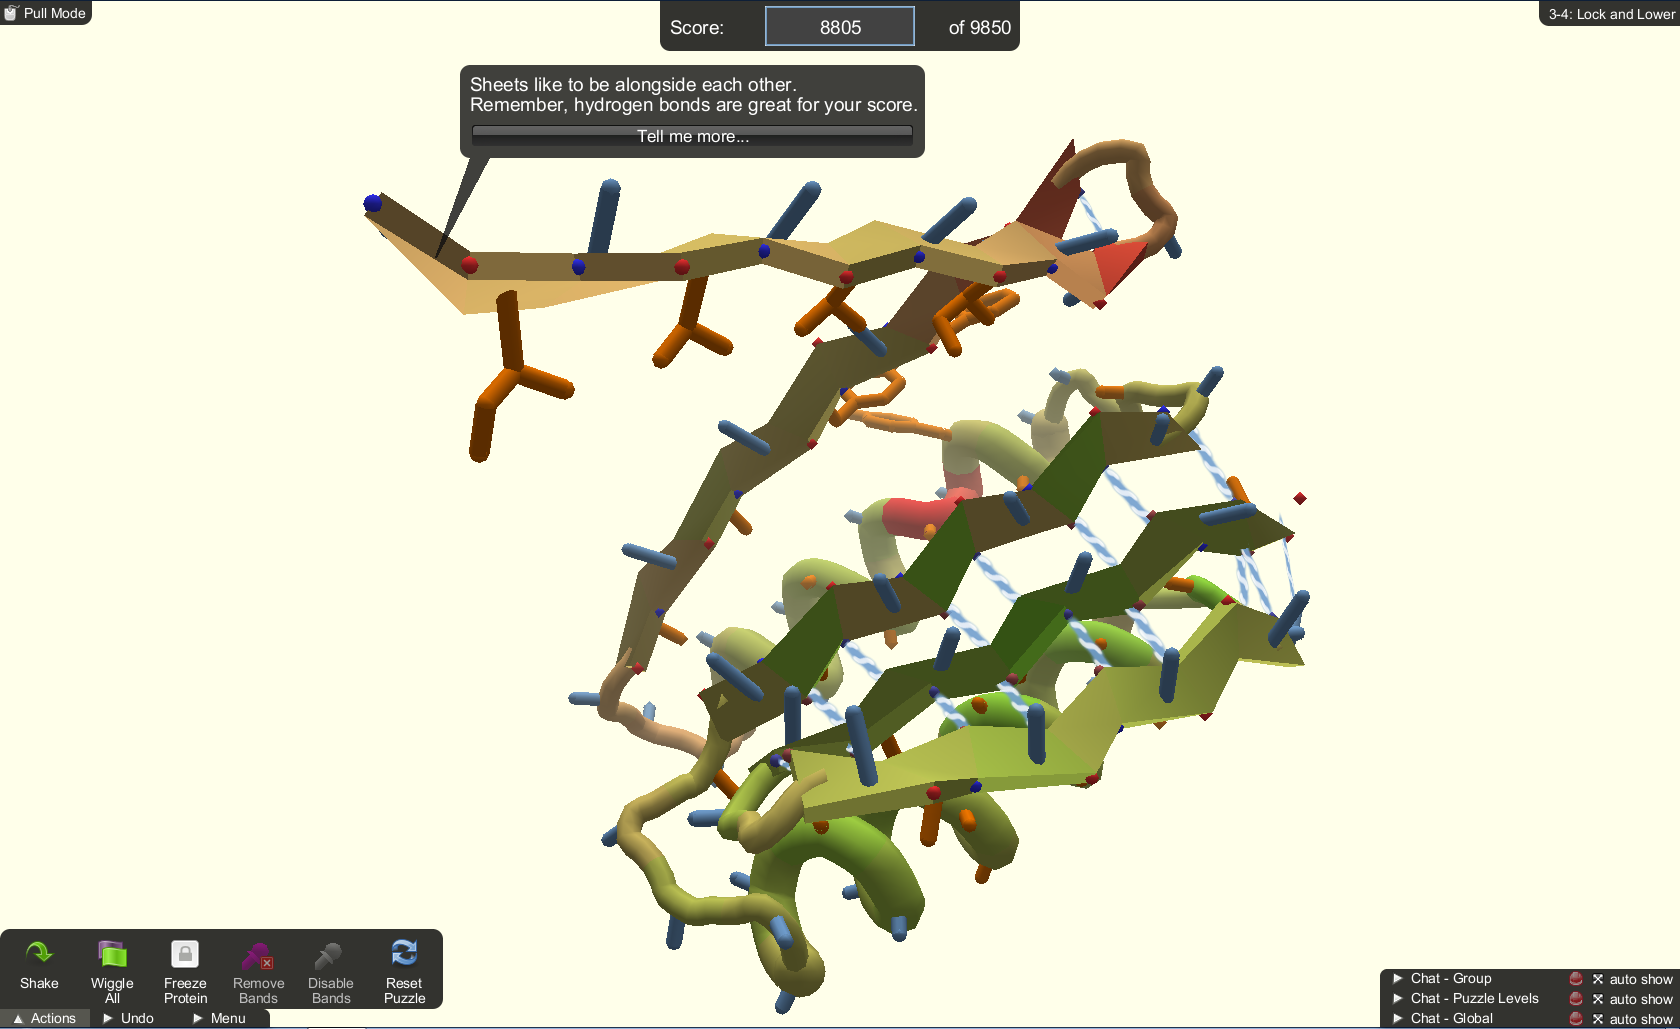
\includegraphics[width=0.8\columnwidth]{foldit.eps}
		\caption{Foldit is solving a serious problem}
		\label{fig:foldit}
\end{figure}

Serious Alternative Reality Game (ARG) is one type of serious game that blends the real and virtual worlds activities in the serious gaming context. Jane McGonigal designed the award winning serious ARG games ``World Without Oil'' \cite{worldwithoutoil} and ``Evoke'' \cite{urgentevoke} with the goal to empower people to come up with creative solutions to our most urgent real-world problems. 

ARGs have also been used to support learning. Connolly et al. \cite{connolly2009arguing} discuss the development of an educational ARG to motivate secondary school students across Europe to learn foreign languages . The results of the pilot run of the game in 2009 indicated that 92\% of students felt the game motivated them to learn a second language. One of problems the team identified is the limitation of Moodle platform the game is based on and there are potentials to improve the effectiveness of the game.

The report of the ARGOSI project \cite{whitton2009alternate} provides insights to the use of ARGs in game based learning and the challenges in the field of higher education. The pilot was run at the University of Bolton with the aim to provide an engaging alternative to traditional methods of introducing students to university life. The overall up-take of the game was fairly low with 173 players and 23 (13\%) of whom were active. The project identifies a number of questions surrounding educational ARGs, such as motivation, relationship to curriculum, marketing and timing. The report
suggests that a complete ARG model may not be appropriate for wholesale learning, but there is certainly potential in using game elements.

While ``Serious Games'' has been an active research topic for decades, ``Gamification'', on the other hand, is a fairly new subject. Deterding et al. \cite {Deterding2011mt} defines gamification is ``the use of game design elements in non-game contexts''. The term only came into widespread use starting in the recent year of 2010 \cite {schell2010design}. Gartner \cite {gartnerPress2011} predicts that by 2015, more than half of companies managing innovation processes will employ gamification, a process of applying game mechanics to application areas including productivity, finance, health, sustainability, news, user-generated content and e-learning. 

FourSquare \cite{foursquare} is probably the most recognized example of applying game mechanics to location-based networking application. It is a location-based game-like service where players check-in to locations for virtual points and rewards.  By employing gamification elements such as points, badges, levels and leader boards, it engages users to revisit a location such as restaurant or pub and become a loyal customer and finally the ``mayor'' of the place. Certain virtual rewards such as the ``mayors'' of Starbucks and badges can be converted into real products, e.g. a free coffee. Foursqure proved that simple game mechanics can affect user behavior by engaging 10 million customers with a successful business model.

\begin{figure}[htbp]
	\centering
		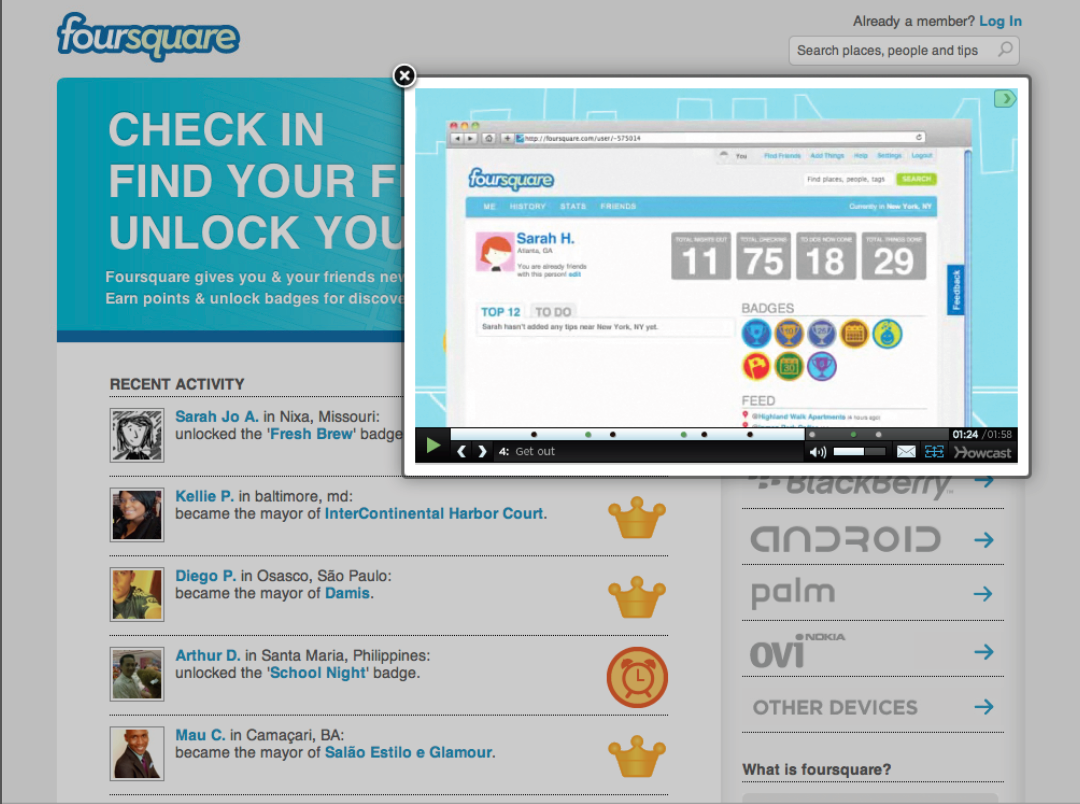
\includegraphics[width=0.7\columnwidth]{foursquare.eps}
		\caption{Foursquare makes modern badges popular}
		\label{fig:foursquare}
\end{figure}

Nike+ \cite{nikeplus}, as another gamification example, is a social running game that employs game mechanics to encourage runners - both casual and hardcore - to compete and improve their fitness, with the goal to solve the main problem of most fitness programs: motivation. Nike+ makes it easy for runners to upload their exercise data to its web site, and start challenging themselves and their friends. They can also get supports from their friends through the web site. The game makes running and exercise fun, which eventually serve the ``serious'' purpose of making players healthy.

\begin{figure}[htbp]
	\centering
		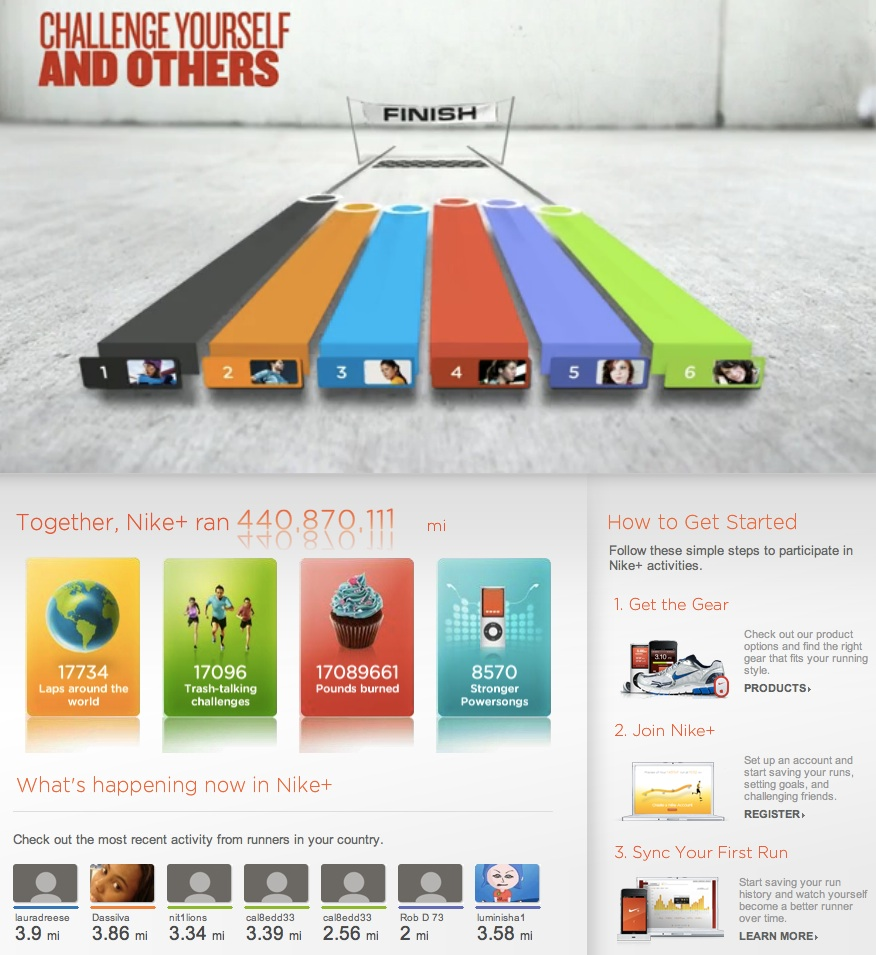
\includegraphics[width=0.6\columnwidth]{nikeplus.eps}
		\caption{Nike+ makes fitness run}
		\label{fig:nikeplus}
\end{figure}

RibbonHero \cite{ribbonhero} is a game that helps users discover new Microsoft Office features in a fun and motivating way. The goal is to have users build familiarity and expose them to the Office UI, so that they understand what kind of features are available. According to the creator of the game, Office ``has a lot of powerful features that users might not know but can be really useful''. The game gives users a chance to learn those features in a fun and engaging way, rather than reading the software manuals or watching the typically dry IT training videos.

\begin{figure}[htbp]
	\centering
		\subfigure[Quest to earn points]{\label{fig:Ribbon1}\includegraphics[height=2.5in]{ribbon1.eps}}
		\subfigure[Competing a task]{\label{fig:Ribbon2}\includegraphics[height=2.5in]{ribbon2.eps}}
		\caption{RibbonHero Helps to Learn Office}
		\label{fig:ribbon}
\end{figure}

Why games? Results of a study published in the May 1998 issue of Nature \cite {koepp1998evidence} demonstrated that video game players experienced regular releases of dopamine during game play. Dopamine is a neurotransmitter that signals pleasure rewards for food, sex and addictive drugs, such as cocaine. 

A favorite subject of the Greek vase-paintings in the ancient games exhibition in the British Museum's department of Greek and Roman antiquities is Ajax and Achilles playing a kind of board game called backgammon, as illustrated in Figure \ref{fig:ancient-games}. It is noteworthy that both Ajax and Achilles have the full armor on while playing the game. According to Arthur A. Krentz \cite{krentz1998play}, in Plato's ``Republic'', the term ``paideia" (in Greek, means education/culture), ``paidia" (means play/game/pastime/sport), and ``paides" (means children), have the same root. The three terms often show up in the same context. ``The central aim of pedagogy (paidagogia) is to encourage learning as a form of play (paidia), which is the most persuasive and effective approach to learning" .

\begin{figure}[htbp]
	\centering
		\includegraphics[width=0.4\columnwidth]{roman-game-vase.eps}
		\caption{Ancient Games Shown in British Museum}
		\label{fig:ancient-games}
\end{figure}

In modern day, World of Warcraft (WoW) is a massively multiplayer online role-playing game (MMORPG) with 11.1 million subscribers, currently the world's most popular MMORPG.  Nick Yee \cite {yee2002understanding} pointed out that the shared experience, the collaborative nature of most activities makes MMORPG unique. ``It's the people that are addictive, not the game''. ``Most importantly, it is the reward of being socialized into a community of gamers and acquiring a reputation within it''  . He claimed \cite {yee2001vsb} that ``WoW truly is a virtual Skinner box'', smoothly increasing reward and difficulty and reinforcing player commitment along the way.
	
In her popular and inspiring TED talk ``Gaming can make a better world" \cite {mcgonigal2010ted} and in her book ``Reality is Broken" \cite {mcgonigal2011reality}, researcher and game designer Jane McGonigal illustrated why good games make us better, and how they can help us change the world. She notes that currently more than 3 billion hours a week is spent in playing video game by our society, for good reasons. She says that the average gamer plays 10,000 hours of games by age 21. That's about the same number of hours that students spent in high school and middle school. There are 500 million gamers today, playing on all sorts of platforms from the iPhone to the game consoles. Instead of the common conception that gaming is a waste of time, she argues that ``playing games is the single most productive thing we can do with our time'' and is the solution to the ``Broken Reality". 

Deterding et al. \cite{Deterding2011mt} describes the distinctions between gamification, serious games and other related concepts, as shown in Figure \ref{fig:define_gamification}. According to Deterding, a) Gamification is about game. It is different than playful interaction, playful design. b) Gamification uses game elements. It is not the complete game such as a serious game. c) Gamification applies to non-game context. Similar to serious game, it uses game for other purposed than game's normal expected use for entertainment. d) Gamification focuses on design. It is not game-based technology or practice of wider game ecology.

\begin{figure}[htbp]
	\centering
		\includegraphics[width=0.5\columnwidth]{defining_gamification.eps}
		\caption{Serious Game and Gamification (source: Deterding \cite{Deterding2011mt})}
		\label{fig:define_gamification}
\end{figure}

While they are different, both gamification and serious games are trying to solve problems with game thinking. Gamification's main driving force is motivation, similarly, serious games also try to solve the motivation problem and influence people's behavior for ``serious'' purpose.  Bosch \cite{bosch2011} considered the serious game Foldit as a victorious example of gamification in science.

\section{Serious Games for Sustainability}

Serious games for sustainability is the games designed to achieve the serious goal of sustainability development.  Reeves et al. \cite{Reeves2011powerhouse} described the design of Power House, an energy game that connects home smart meters to an online multiple player game with the goal to improve home energy behavior. In the game, the real world energy data are transformed into a ``more palatable and relevant form of
feedback'', and players may be incentivized by the in-game rewards to complete more energy-friendly real-world behaviors.

\begin{figure}[htbp]
	\centering
		\includegraphics[width=0.8\columnwidth]{powerhouse.eps}
		\caption{Power House Game to Save Energy(source: Reeves \cite{Reeves2011powerhouse})}
		\label{fig:powerhouse}
\end{figure}

RecycleBank \cite {recyclebank} introduced a series of ``Green Challenges'' that used gaming techniques online to motivate participants to learn about green living and to take small green actions to live more sustainable lives offline. According to this report \cite {gamingforgood}, 49,000 individuals participated in the ``Green Your Home Challenges''. Partnered with Google Analytics and ROI research, they found that:
\begin{itemize}
	\item Gamification can increase awareness of positive environmental actions. 97\% of participants surveyed said the game increase their knowledge of environment.
	\item Games can drive individuals to take positive social and environmental actions. Most participants surveyed indicated they are very or extremely likely to take green actions as a result of participating in the challenge.
	\item Games are an effective and appealing educational tool. 86\% participants agreed online games and contest can be a good way to inform and educate them personally.
\end{itemize}

\begin{figure}[htbp]
	\centering
		\subfigure[Green Your Home Challenge]{\label{fig:RecycleBank1}\includegraphics[width=0.7\columnwidth]{recyclebank1.eps}}
		\subfigure[Game Change Behavior]{\label{fig:RecylceBank2}
\includegraphics[width=0.7\columnwidth]{recyclebank2.eps}}
		\caption{RecycleBank - Gaming for Good}
		\label{fig:recyclebank}
\end{figure}

Interactive design also applies game elements in their design to achieve sustainability goal. The ``SmartGauge'' dashboard \cite {ideo2009} for Ford's hybrid cars, where a digital plant is responding to how energy-efficient the users driving behavior is. The design gives drivers a game, with the goal to grow more lush and beautiful leaves, a visual reward, by driving efficiently, thus promotes a more environmental behavior. Similarly, The design of ``Piano Staircase'' \cite {funtheory2009}, created by Volkswagen Sweden, installed in a metro station in Stockholm, is to make the staircase next to the escalator look and respond like a piano keyboard, so that every step on the stair will generate different piano sounds every time a commuter walked on it. Observation indicates that 66 percent more people chose to play the ``piano staircase'' game over using the escalator. It is a good example of gameful design for persuading and encouraging energy-efficient behavior.

 \begin{figure}[htbp]
	\centering
		\subfigure[Efficiency Leaves]{\label{ixd-dashbard}\includegraphics[width=0.7\columnwidth]{ixd-dashboard.eps}}
		\subfigure[Piano Stair vs. Escalator]{\label{fig:ixd-pianostair}\includegraphics[width=0.7\columnwidth]{ixd-pianostair.eps}}
		\caption{Gameful Design for Sustainability}
		\label{fig:ixd}
\end{figure}	

Energy competitions or challenges have been introduced to college dormitories and residential homes as ways to facilitate and incentivize energy reduction. Petersen et al. \cite{petersen-dorm-energy-reduction} describe their experiences deploying a real-time feedback system in an Oberlin College dorm energy competition in 2005 that includes 22 dormitories over a 2-week period. They found a 32\% reduction in electricity use across all dormitories. However, in a post-competition survey, respondents indicated that some behaviors, such as turning off hallway lights at night and unplugging vending machines were not sustainable outside the competition period.  There has been little analysis on energy usage after competitions finish, or how positive behavior changes could be sustained.

\begin{figure}[htbp]
	\centering
		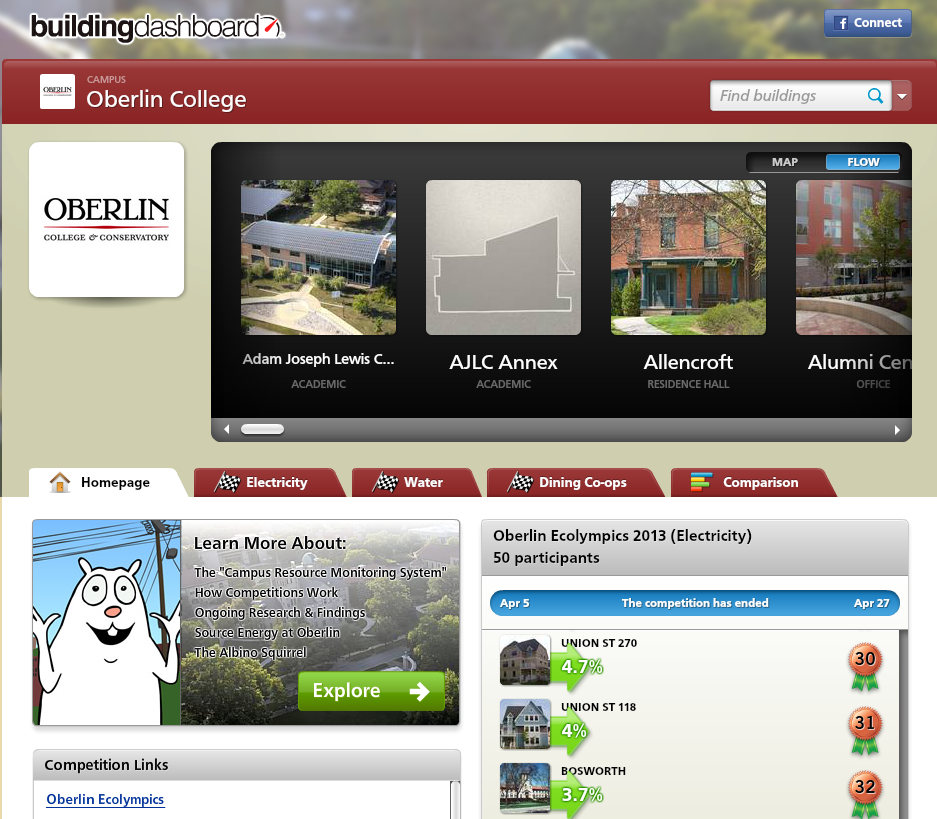
\includegraphics[width=0.7\columnwidth]{oberlin.eps}
		\caption{Energy Competition for Sustainability}
		\label{fig:oberlin}
\end{figure}

\section{Serious Game Frameworks}

Game frameworks (also known as game engines) \cite{sherrod2006ultimate} are ``comprised of a collection of different tools, utilities, and interfaces that hide the low-level details of the various tasks that make up a game''. The examples of game frameworks include:
\begin {itemize}
    \item Unreal \cite{unrealengine}:  The Unreal Engine is a game engine developed by Epic Games, it is primarily used in first person shooter games, providing tools and building blocks for 3D rendering, collision detection, AI, networking etc.
    \item PapayaMobile \cite{papayamobile}: PapayaMobile is a free cross platform social game engine on Android and iOS platform. It provides an SDK and a platform for mobile game developers to create and release games in a ``user-friendly, straightforward way''.
    \item OpenLabyrinth \cite{openlabyrinth}: OpenLabyrinth is an open source game framework that allows its users to create, run and analyze a wide range of different pathway-based activities for healthcare education.
    \item Fabula \cite{fabula}: Fabula is an open source Python game engine for adventure, role-playing and strategy games and digital interactive storytelling. It provides a library and game world abstraction intuitive to people who have not been involved in game development before and hide as much as lovel level technical details as much as possible.
\end {itemize}

One of the benefits of using a game framework is that, if correctly designed, it will provide useful and reusable ``building blocks'' with which to develop a variety of games. Similarly, Serious game frameworks also provide building blocks that enable the serious game developer to focus more time and thought on content and results instead of on the technical details and infrastructure for creating the serious game.

There are two serious game frameworks related to sustainability development. One such framework is the Building Dashboard \cite{building-dashboard}, developed by Lucid Design Group, as shown in Figure \ref{fig:building-dashboard}.

\begin{figure}[htbp]
	\centering
		
\includegraphics[width=0.6\columnwidth]{building-dashboard.eps}
		\caption{Building Dashboard (source: Lucid \cite{building-dashboard})}
		\label{fig:building-dashboard}
\end{figure}

Building Dashboard is commercial platform that ``enables energy reduction competition and empowers building occupants to become active participants in energy management''. It is used to support the Campus Conservation Nationals (CCN) \cite{competetoreduce}, a nationwide electricity and water use reduction competition on college campuses. In CCN 2014, the framework was used by 109 schools in north american to display the energy and water consumption to the competition participants. It enables viewing, comparing and sharing building energy
and water use information on the web in compelling visual interface, but the
cost of the commercial system creates the barrier for wider adoptions. In addition, the
building dashboard solutions focus on providing energy information as
a passive media. Besides a scoreboard, There is little interaction between participants
and the system.

Another framework that is related to sustainability development is the Stanford Energy Services Platform \cite{Armel-2012}, as shown in Figure \ref{fig:stanford-platform}. It provides services to benefit the creations of energy efficiency program and research. The services include data storage, recommendation system, user registration and participation assignment, surveys and analytics. It had been utilized to support
the implementation of several Stanford's energy saving projects and energy related serious games, such as Power House game, Power Down game, and Energy Calculator. At this point, there is not enough information about the Stanford Energy Services Platform regarding the availability and features. 

\begin{figure}[htbp]
	\centering
		\includegraphics[width=0.6\columnwidth]{stanford-esp.eps}
		\caption{Stanford Energy Services Platform (source: Stanford \cite{Armel-2012})}
		\label{fig:stanford-platform}
\end{figure}
 
%% TODO: add non-serious game framework assessment
\section{Serious Game Framework Assessment}
\label{Serious-Game-Framework-Assessment}

This section examines the assessment of serious game frameworks. It starts with looking at the assessment of serious games, then looks at the assessment of game frameworks in general, finally examines the assessment of serious game frameworks in particular.

One fundamental question in evaluating a serious game is the extent to which the
game achieves its ``serious'' purpose.  This is quite different from 
traditional entertainment games, in which evaluation focuses on usability or
playability \cite{song2007new}. In the field of serious games, there is an increasing
focus on the methodology of game evaluation \cite{Mayer2012233}. 

De Freitas and Oliver \cite{de2006can} pointed out that there are few frameworks to support the evaluation of education games. They introduced the four dimensional framework for evaluating 
educational games and simulations. The framework consisting of: the context, the pedagogy, the representation, and the learner (or player). Figure \ref{fig:four-dimensional-framework} illustrates the evaluation framework.

\begin{figure}[htbp]
	\centering
		\includegraphics[width=0.7\columnwidth]{game-eval.eps}
		\caption{Four Dimensional Framework for Evaluating Educational Games \cite{de2006can}}
		\label{fig:four-dimensional-framework}
\end{figure}

Harteveld \cite{harteveld2010triadic} also agrees that ``Evaluatory research for games with a serious purpose is still at its infancy''. He proposes an evaluation framework called ``Triadic Game Evaluation (TGE)'' for assessing serious games. It consisting of three perspectives: Reality,
Meaning, and Play, as illustrated in the Figure \ref{fig:triadic-game-eval}.

\begin{figure}[htbp]
	\centering
		\includegraphics[width=0.7\columnwidth]{triadic-eval.eps}
		\caption{Triadic Game Evaluation (TGE) \cite{harteveld2010triadic}}
		\label{fig:triadic-game-eval}
\end{figure}

The above approaches focus on evaluation of a single game, as opposed to a game {\em
  framework}. One of the benefits of using a game framework is that, if correctly designed, it will provide useful and reusable ``building blocks'' with which to develop a variety of games. Yet how are we to know if a game framework has been ``correctly designed''?

Berger and Muller \cite {fabulaengine} described their approach of using the Technology Acceptance Model (TAM) to evaluate the custom game engine Fabula \cite{fabula}. Technology Acceptance Model \cite {davis1986technology} is a well received theoretical model on assessing user acceptance of computer-based information systems, introduced by Fred Davis in his doctoral thesis in 1985. TAM considers that system use is a response that can be predicated by user motivation, which is influenced by an external stimulus of the system's features and capabilities. Figure \ref{fig:tam} illustrates the original Davis model. X1, X2 and X3 in the figure represent the system features.

\begin{figure}[htbp]
	\centering
		\includegraphics[width=0.7\columnwidth]{tam.eps}
		\caption{Technology Acceptance Model (TAM) \cite{davis1986technology}}
		\label{fig:tam}
\end{figure}

As Chuttur \cite{chuttur2009overview} pointed out in his review of TAM that there are skepticisms among some researchers regarding the rigor and limitations of the model. There exists some other assessment tools such as Game Engagement Questionnaire (GEQ) and Questionnaire for User Interaction Satisfaction (QUIS).  

Game Engagement Questionnaire (GEQ) \cite{brockmyer2009development} was developed by Brockmyer et al. and published in the Journal of Experimental Social Psychology. The questionnaire provides a ``psychometrically'' strong measure of levels of engagement specifically while playing video games. While the GEQ could measure the engagement level of positive game experience, the orignal intent of the research is to ``examine risk and protective factors for negative game impact''. Figure \ref{fig:geq} shows the questionnaire items.

\begin{figure}[htbp]
	\centering
		\includegraphics[width=0.7\columnwidth]{geq.eps}
		\caption{Game Engagement Questionnaire (GEQ) items \cite{brockmyer2009development}}
		\label{fig:geq}
\end{figure}

Questionnaire for User Interaction Satisfaction (QUIS) \cite{harper1993improving} is a usability assessment tool developed in the HCI lab at the University Of Maryland, College Park. It is designed to assess user's subjective satisfaction regarding the human/computer interface of software systems. Currently licensing is required to access the QUIS questionnaires. 

The above assessment framework or tools are for general purpose. From my literature search, I have not yet found any prior work concerning the comprehensive approach for the particular needs of a serious game framework assessment. 